\chapter{Конструкторская часть}

В данном разделе представлены этапы проектирования баз данных и OLAP Cube.

\section{Проектирование отношений сущностей}

На рисунках \ref{fig:ER-Chen} и \ref{fig:ER-App} представлены ER диаграммы сущностей, необходимых для реализации приложения.

\newpage

\begin{figure}[!h]
	\center{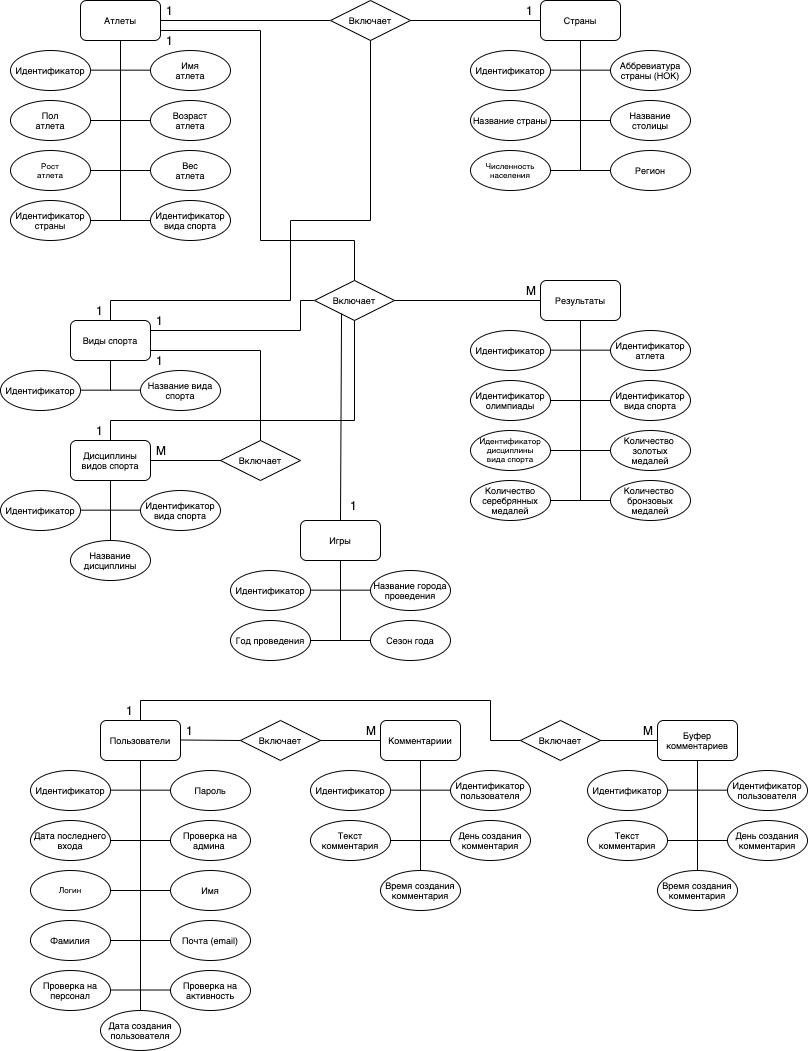
\includegraphics[scale=0.6]{img/er-chen.png}}
	\caption{ER-диаграмма сущностей базы данных в нотации Чена}
	\label{fig:ER-Chen}
\end{figure}

\begin{figure}[!h]
	\center{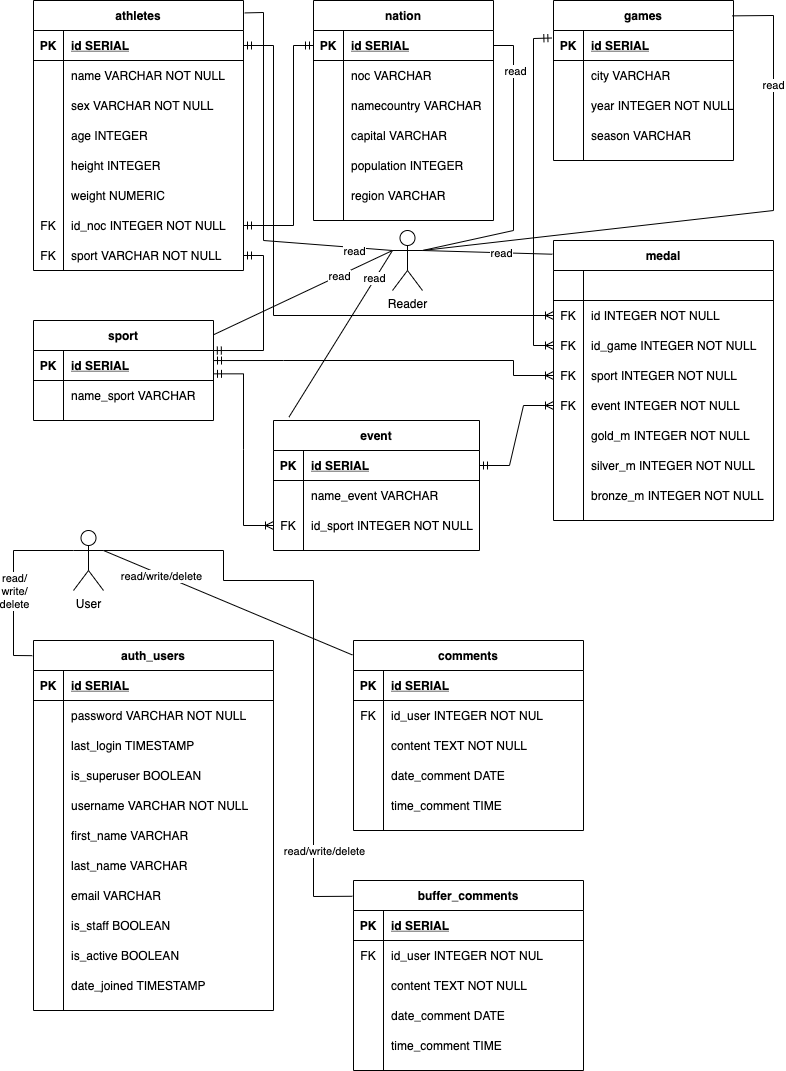
\includegraphics[scale=0.6]{img/er.png}}
	\caption{ER диаграмма сервиса}
	\label{fig:ER-App}
\end{figure}


\newpage
\section{Проектирование базы данных Олимпийских игр}

База данных будет реализована с использованием СУБД PostgreSQL. В базе данных будет существовать 9 сущностей и 9 таблиц. ER-диаграма сущностей этой базы данных представлена на рисунке \ref{fig:ER-App}.

Поля таблицы \texttt{athletes} означают:

\begin{itemize}
	
	\item  \texttt{id} - уникальный идентификатор спортсмена;
	
	\item  \texttt{name} - имя спортсмена;
	
	\item  \texttt{sex} - пол спортсмена. Поле принимает значение М или F, 
	если пол спортсмена мужской или женский соответсвенно;
	
	\item  \texttt{age} - возраст спортсмена;
	
	\item  \texttt{height} - рост спортсмена с точностью до см;
	
	\item  \texttt{weight} - вес спортсмена с точностью до 0.1 кг;
	
	\item  \texttt{id\_noc} - идентификатор страны спортсмена;
	
	\item  \texttt{sport} - идентификатор вида спорта, которым занимается спортсмен;
	
\end{itemize}


Поля таблицы \texttt{nation} означают:

\begin{itemize}
	
	\item  \texttt{id} - уникальный идентификатор страны;
	
	\item  \texttt{noc} - аббревиатура страны (НОК);
	
	\item  \texttt{namecountry} - полное название страны;
	
	\item  \texttt{capital} - город, являющийся столицей страны;
	
	\item  \texttt{population} - количество населения;
	
	\item  \texttt{region} - регион (часть света), в котором расположена страна;
	
\end{itemize}


Поля таблицы \texttt{games} означают:

\begin{itemize}
	
	\item  \texttt{id} - уникальный идентификатор Олимпиады;
	
	\item  \texttt{city} - город, в котором проходила Олимпиада;
	
	\item  \texttt{year} - год прохождения олимпиады;
	
	\item  \texttt{season} - сезон года, в котором проходила Олимпиада. 
	Может принимать значения Summer или Winter, если Олимпиада была летом или зимой соответственно;
	
\end{itemize}

Поля таблицы \texttt{sport} означают:

\begin{itemize}
	
	\item  \texttt{id} - уникальный идентификатор вида спорта;
	
	\item  \texttt{name\_sport} - название вида спорта;
	
\end{itemize}

Поля таблицы \texttt{event} означают:

\begin{itemize}
	
	\item  \texttt{id} - уникальный идентификатор дисциплины вида спорта;
	
	\item  \texttt{name\_event} - название дисциплины вида спорта;
	
	\item  \texttt{id\_sport} - идентификатор вида спорта, которому принадлежит дисциплина;
	
\end{itemize}

Поля таблицы \texttt{medal} означают:

\begin{itemize}
	
	\item  \texttt{id} - идентификатор спортсмена;
	
	\item  \texttt{id\_game} - идентификатор Олимпиады;
	
	\item  \texttt{sport} - вид спорта в котором принимал участие спортсмен;
	
	\item  \texttt{event} - дисциплина а в которой соревновался спортсмен;
	
	\item  \texttt{gold\_m} - количество золотых медалей, которое спортсмен выиграл за участие в данной дисциплине на этой Олимпиаде (может быть 0 или 1, если не выиграл или выиграл соответственно);
	
	\item  \texttt{silver\_m} - количество серебрянных медалей, которое спортсмен выиграл за участие в данной дисциплине на этой Олимпиаде (может быть 0 или 1, если не выиграл или выиграл соответственно);
	
	\item  \texttt{bronze\_m} - количество бронзовых медалей, которое спортсмен выиграл за участие в данной дисциплине на этой Олимпиаде (может быть 0 или 1, если не выиграл или выиграл соответственно);
	
\end{itemize}

Поля таблицы \texttt{auth\_user} означают:

\begin{itemize}
	
	\item  \texttt{id} - уникальный идентификатор пользователя;
	
	\item  \texttt{password} - захэшированный пароль;
	
	\item  \texttt{last\_login} - дата, последней авторизации пользователя в сервисе;
	
	\item  \texttt{is\_superuser} - проверка того, что пользователь является админом (может принимать значение true, если является, иначе false);
	
	\item  \texttt{username} - логин пользователя, должен быть уникальным для каждого;
	
	\item  \texttt{first\_name} - имя пользователя;
	
	\item  \texttt{last\_name} - фамилия пользователя;
	
	\item  \texttt{email} - почта пользователя;
		
	\item  \texttt{is\_staff} - проверка того, что пользователь является одним из сотрудников сервиса (может принимать значение true, если является, иначе false);
	
	\item  \texttt{is\_active} - проверка того, что пользователь ещё пользуется сервисом;
	
	\item  \texttt{data\_joined} - дата созлания аккаунта пользователя;
	
\end{itemize}




Поля таблицы \texttt{comments} означают:

\begin{itemize}

\item  \texttt{id} - уникальный идентификатор комментария;

\item  \texttt{id\_user} - идентификатор пользователя, оставившего комментарий;

\item  \texttt{content} - текст комментария;

\item  \texttt{date\_comment} - дата публикации комментария (год, месяц, день);

\item  \texttt{time\_commen} - время публикации комментария (час, минута, секунда);

\end{itemize}

Таблица \texttt{buffer\_comments} является полной копией таблицы \texttt{comments}. Данная таблица содержит все комментарии, которые когда-либо были добавлены пользователями и предназаначина только для нужд администратора. Если удалить комментарий из таблицы  \texttt{comments}, то в таблице \\  \texttt{buffer\_comments} он останется без изменений.

\section{Проектирование отношений между таблицей фактов и измерений  в OLAP Cube}

Развёрнутый OLAP Cube будет содержать таблицу фактов, по которой будет происходить поиск мер по заданным параметрам и  их агрегирование. Операции с OLAP моделью (drilldown, slice, dice и другие) будут возможны благодаря рабиению таблицы фатков по осям (измерениям).

\newpage
Компоненты проектируемого OLAP куба:

\begin{itemize}
	
	\item  В качестве таблицы фактов \cite{cube-operations} принимается таблица \texttt{medal};
	
	\item  В качестве осей (измерений)  \cite{cube-operations} принимаются таблицы: \texttt{athletes}, \texttt{nation}, \texttt{games}, \texttt{sport} и \texttt{event};
	
	\item  В качестве мер агрегации  \cite{cube-operations} принимаются поля таблицы \texttt{medal}: \texttt{gold\_m}, \texttt{silver\_m}, \texttt{silver\_m};
	
	\item  Связь измерений с таблицей фактов реализуется благодаря отношению \texttt{left-join} \cite{cube-schemas}, поддерживаемого OLAP системами;
	
\end{itemize}


\section*{Вывод}

В данном разделе были представлены этапы проектирования базы данных и OLAP Cube, а также показана ER диаграмма сервиса.


